
The previous chapter gave insight into the problem and some variants, but left most of the harder questions open.
This chapter will serve as a finite check of the results and conjectures by testing them on small graphs through brute-force enumeration.
It will also be the foundation of conjectures for the open cases, by discovering extremal graphs or at least sufficiently dense graphs.
Pattern recognition on the discovered values, or even a family of extremal graphs, then lets conjectures be made, although those statements are naive because they are based on small graphs only.
Larger graph spaces will be scoured by a heuristic, namely tabu search.
A guided search is needed there because only a small fraction of the search space is extremal: assigning edges at random gives a binomially distributed edge count, so almost every graph lands far from the cap.
The archive is the repository at \url{https://github.com/louisvandenbruwaene/thesis} and every file path quoted in this thesis is relative to it, or to a base directory named where the path is given, with the commands and the audit trail collected in \Cref{sec:transcripts}.
Below is a diagram of the program's architecture, showing how the modelled graphs are fed to the checker and how the results are used to either certify or discover bounds.
\begin{figure}[ht]
\centering
\spinediagram
\caption{A single model feeds the exact max-flow checker. Certification turns that measurement into finite upper bounds, while heuristic search uses it to discover lower bounds. The badge colours on the code cards match the boxes here.}
\label{fig:spine}
\end{figure}

\section{Modelling}
All non-hypergraphs are represented using one multiplicity matrix $\mu$: it is symmetric when undirected and binary when simple.
Hypergraphs are stored as (multi)sets of hyperedges, which are sets of vertices with a tail distinguished in the directed model.
\Cref{fig:matrix-rep} shows this encoding for a directed multigraph and hypergraph.
Matrix or tensor representations for hypergraphs are thus not recommended due to their size and sparsity.
All possible graphs of a given size will later be checked to see if they are extremal for the given size and connectivity restraint.
Matrices are iterated as a depth-first search with entries in $\{0,1\}$ for simple graphs and in $\{0,\ldots,m-1\}$ for multigraphs, and the diagonal is always zero.
Hypergraphs are implemented similarly from the ground up as there are no matrix tools for them.
Notice how depth-first search is memory-efficient.


\section{Measuring}
Given $n$ and $m$, walk through every graph on $n$ vertices, measure the largest
local connectivity $\lambda^{\max}$ or $\kap^{\max}$ of each with a max-flow computation and
keep the densest graph that stays at or below the cap $m - 1$.
If the enumeration cannot finish within the time limit, the best graph so far is returned.
It is therefore important to distinguish between the densest graph possible and the densest graph found.
A completed enumeration gives an exact extremal value. An unfinished enumeration gives only a lower bound.
In the vertex-disjoint and hypergraph cases the graph will be transformed before the flow can be measured.
This ensures that every variant shares the same integer max-flow engine no matter the implementation.
Thus the whole question reduces to a flow computation:
A \emph{maximum flow} asks how much can be pushed from one point to another through a network whose links each carry a limited capacity.
Menger's theorem (\Cref{thm:menger}) already turned $\lambda(u,v)$ into the number of edges/arcs in a minimum cut.
For a simple graph, $\lambda(u,v)$ is therefore also the capacity of a cut over a network with unit capacities.
For a multigraph, the parallel copies can be combined into one link whose capacity is their multiplicity $\mu(u,v)$.
In the directed case these capacities follow the direction of the arcs, while in the undirected case they are available in either direction.
The max-flow/min-cut theorem of Ford and Fulkerson \cite{FordFulkerson56} says that this smallest cut has exactly the value of a maximum flow.
So the route count we are after is just a maximum-flow value: measure the flow and you have measured the connectivity.

The routine that runs this flow and reports the route count is the connectivity \emph{checker}.
The program ships an optional compiled C helper that runs this same flow more efficiently.

\subsection{Transformations}
This max-flow computation is built for directed multigraphs (including simple digraphs) with edge-disjoint paths.
That is why the other variants will have to be transformed into such a flow network.
Undirected multigraphs have a natural identification with a directed multigraph, obtained by replacing every edge with a pair of arcs going in opposite directions.
To transform a multihypergraph, replace each distinct hyperedge with a helper gate,
an entry point and an exit point joined by a single arc whose capacity is the multiplicity of the hyperedge.
Every member of the hyperedge then flows into the entry and out of the exit at unlimited capacity,
so the one arc between them is the only bottleneck (\Cref{fig:hyper-gadget}).
A directed hyperedge is wired the same way, except that only its tail reaches the entry and only its heads leave the exit,
which is what forces a route to cross it from tail to head.
The directed hypergraph's flow network is just a restricted version of the undirected one.
Another representation for multihypergraphs is a separate gate with capacity one for each hyperedge.

The proposed hypergraph Menger argument (\Cref{thm:menger-hyper}) explains that the resulting maximum flow is exactly the Berge connectivity.
\Cref{fig:hyper-gadget-example} shows four gate-disjoint routes in a whole hypergraph.
For the vertex-disjoint hypergraph checker, only the ordinary vertices are split into unit-capacity gates. Each hyperedge retains its multiplicity-capacity gate.

Lastly, all vertex-disjoint versions can then be transformed into an identical edge-disjoint question by splitting
each vertex $v$ into an in-copy $v^{\mathrm{in}}$ and an out-copy $v^{\mathrm{out}}$ joined by a single unit-capacity arc (\Cref{fig:vertex-split}).
Every arc $u \to v$ of the digraph becomes $u^{\mathrm{out}} \to v^{\mathrm{in}}$ in the split network.
Routing through $v$ now consumes the one unit of capacity on its internal arc,
so two paths sharing $v$ as an intermediate vertex compete for that unit and cannot coexist in any maximum flow.
A max-flow from $u^{\mathrm{out}}$ to $v^{\mathrm{in}}$ in the split network therefore equals the number of internally vertex-disjoint $u$-$v$ paths in the original graph.
For a multigraph the arc carrying an adjacency keeps its full capacity
$\mu(u,v)$, and only the internal arc of a vertex is a unit. That is the
incidence convention of \Cref{sec:incidence-convention} written as a network:
parallel copies stay separate routes while the vertex they run through does not,
so the split network measures $K_m(n)$ and $K_m^{\mathrm{dir}}(n)$ rather than
the value of the underlying simple graph.
Notice how the undirected or hypergraph transformation is done beforehand and
the gates aren't split by this step.

\begin{figure}[htbp]
\centering
% Printed legibility: this picture holds two 8-unit panels side by side, so
% every extra centimetre of gap or of resize headroom is paid for twice over in
% label size. The gap is kept tight, the box is given the full text width, and
% the station and gate fonts are stepped up, which together lift the smallest
% label from about 5.4pt to roughly 9pt on paper.
\resizebox{\textwidth}{!}{%
\begin{tikzpicture}[scale=0.92, >=Stealth,
   metro/.append style={line width=3.0pt},
   metrostop/.append style={font=\small\bfseries, minimum size=6.6mm},
   faded/.style={metro, opacity=0.35, line width=2.2pt},
   flow/.style={line width=1.2pt, black!88, line cap=round,
                preaction={draw, line width=3.0pt, white}},
   gate/.style={circle, fill=white, draw=black!30, line width=0.6pt,
                inner sep=0.4pt, minimum size=13.5pt, font=\small}]
\def\stations{%
  \coordinate (Sa) at (0,0);  \coordinate (Sc) at (2,2);  \coordinate (Sd) at (6,2);
  \coordinate (Se) at (0,4);  \coordinate (Sj) at (8,4);  \coordinate (Sl) at (2,6);
  \coordinate (Sm) at (6,6);  \coordinate (Sn) at (0,8);}
% Every station carries its own letter, since the captions name hyperedges and
% routes by those letters.  The chosen pair also carries its role name, u or v,
% in blue just outside the station.
\def\drawstops{%
  \foreach \id/\lab in {Sa/a,Sc/c,Sd/d,Se/e,Sj/j,Sl/l,Sm/m,Sn/n}
     {\node[metrostop] at (\id) {$\lab$};}
  \node[font=\small\bfseries, text=KULblauw1] at ($(Se)+(-0.62,0.52)$) {$u$};
  \node[font=\small\bfseries, text=KULblauw1] at ($(Sm)+(0.62,0.52)$) {$v$};}
% --- panel (a): the hypergraph, every hyperedge vertex to vertex ---
\begin{scope}
  \stations
  \begin{scope}[on background layer]
    \draw[metro, metroA] (Se) -- (Sa);
    \draw[metro, metroA] (Sa) -- (Sd);
    \draw[metro, metroB] (Sn) -- (Sm);
    \draw[metro, metroB] (Sm) -- (Sj);
    \draw[metro, metroC] ($(Se)+(0.14,-0.14)$) -- ($(Sl)+(0.14,-0.14)$);
    \draw[metro, metroC] (Sl) -- (Sc);
    \draw[metro, metroD] (Se) -- (Sd);
    \draw[metro, metroD] (Sd) -- (Sm);
    \draw[metro, metroF] (Sn) -- (Se);
    \draw[metro, metroF] (Se) -- (Sl);
    \draw[metro, metroH] ($(Se)+(-0.14,0.14)$) -- ($(Sl)+(-0.14,0.14)$);
    \draw[metro, metroH] (Sl) -- (Sm);
    \draw[metro, metroG] (Sm) -- (Sc);
    \draw[metro, metroG] (Sc) -- (Sj);
    \draw[metro, metroE] (Sl) -- (Sd);
    \draw[metro, metroE] (Sd) -- (Sj);
  \end{scope}
  \drawstops
  \node[font=\small] at (4,-1.4) {(a)};
\end{scope}
% --- panel (b): the helper-point flow network for the pair u, v ---
\begin{scope}[xshift=9.6cm]
  \stations
  \coordinate (Helc) at (1,3);
  \coordinate (Hmcj) at (5,4);
  \coordinate (Hedm) at (3,3.7);
  \coordinate (Helm) at (1.6,6.7);
  \coordinate (Hnel) at (0.50,6.00);
  \coordinate (Hnmj) at (3.27,7.81);
  \begin{scope}[on background layer]
    \draw[faded, metroA] (Se) -- (Sa);
    \draw[faded, metroA] (Sa) -- (Sd);
    \draw[faded, metroB] (Sn) -- (Sm);
    \draw[faded, metroB] (Sm) -- (Sj);
    \draw[faded, metroC] ($(Se)+(0.14,-0.14)$) -- ($(Sl)+(0.14,-0.14)$);
    \draw[faded, metroC] (Sl) -- (Sc);
    \draw[faded, metroD] (Se) -- (Sd);
    \draw[faded, metroD] (Sd) -- (Sm);
    \draw[faded, metroF] (Sn) -- (Se);
    \draw[faded, metroF] (Se) -- (Sl);
    \draw[faded, metroH] ($(Se)+(-0.14,0.14)$) -- ($(Sl)+(-0.14,0.14)$);
    \draw[faded, metroH] (Sl) -- (Sm);
    \draw[faded, metroG] (Sm) -- (Sc);
    \draw[faded, metroG] (Sc) -- (Sj);
    \draw[faded, metroE] (Sl) -- (Sd);
    \draw[faded, metroE] (Sd) -- (Sj);
  \end{scope}
  \draw[flow] (Se) -- (Helc);
  \draw[flow] (Helc) -- (Sc);
  \draw[flow] (Sc) -- (Hmcj);
  \draw[flow] (Hmcj) -- (Sm);
  \draw[flow] (Se) -- (Hedm);
  \draw[flow] (Hedm) -- (Sm);
  \draw[flow] (Se) -- (Helm);
  \draw[flow] (Helm) -- (Sm);
  \draw[flow] (Se) -- (Hnel);
  \draw[flow] (Hnel) -- (Sn);
  \draw[flow] (Sn) -- (Hnmj);
  \draw[flow] (Hnmj) -- (Sm);
  % dotted leg from each gate to the hyperedge's unused third member
  \draw[densely dotted, line width=1pt, opacity=0.7, shorten >=3mm, metroC] (Helc) -- (Sl);
  \draw[densely dotted, line width=1pt, opacity=0.7, shorten >=3mm, metroG] (Hmcj) -- (Sj);
  \draw[densely dotted, line width=1pt, opacity=0.7, shorten >=3mm, metroD] (Hedm) -- (Sd);
  \draw[densely dotted, line width=1pt, opacity=0.7, shorten >=3mm, metroH] (Helm) -- (Sl);
  \draw[densely dotted, line width=1pt, opacity=0.7, shorten >=3mm, metroF] (Hnel) -- (Sl);
  \draw[densely dotted, line width=1pt, opacity=0.7, shorten >=3mm, metroB] (Hnmj) -- (Sj);
  \node[gate] at (Helc) {$h_{\textcolor{metroC}{\bullet}}$};
  \node[gate] at (Hmcj) {$h_{\textcolor{metroG}{\bullet}}$};
  \node[gate] at (Hedm) {$h_{\textcolor{metroD}{\bullet}}$};
  \node[gate] at (Helm) {$h_{\textcolor{metroH}{\bullet}}$};
  \node[gate] at (Hnel) {$h_{\textcolor{metroF}{\bullet}}$};
  \node[gate] at (Hnmj) {$h_{\textcolor{metroB}{\bullet}}$};
  \drawstops
  \node[font=\small] at (4,-1.4) {(b)};
\end{scope}
\end{tikzpicture}}
\caption[The helper-point network on a whole hypergraph]{An undirected $3$-uniform hypergraph and its gate network for $u,v$. The four black routes use distinct capacity-one gates (they are drawn as one point to reduce visual clutter), so the checker reads $\lec(u,v)=4$. A fifth would reuse a gate. The helper points connect to the hyperedge's third member by dotted lines.}
\label{fig:hyper-gadget-example}
\end{figure}

% Printed legibility: three panels across at 0.32\textwidth shrank each picture
% to roughly 0.58 of natural size and its labels to under 5pt. Stacking them
% one per row at 0.70\textwidth reverses that, drawing each slightly larger
% than natural instead.
\begin{figure}[ht]
\centering
\begin{subfigure}[b]{0.70\textwidth}
\centering
\resizebox{\linewidth}{!}{%
\begin{tikzpicture}[>=Stealth]
\node[vertex] (v) at (1.0, 0) {$v$};
\draw[->, edge] (0.0,  0.6) -- (v);
\draw[->, edge] (0.0, -0.6) -- (v);
\draw[->, edge] (v) -- (2.0,  0.6);
\draw[->, edge] (v) -- (2.0, -0.6);
\draw[->, very thick, color=KULblauw3b] (2.8, 0) -- (3.8, 0);
\node[smallvertex, minimum size=8mm] (vi) at (5.0, 0) {$v^{\mathrm{in}}$};
\node[smallvertex, minimum size=8mm] (vo) at (7.0, 0) {$v^{\mathrm{out}}$};
\draw[->, edge, color=KULblauw3b] (vi) -- node[above, font=\scriptsize]{capacity $1$} (vo);
\draw[->, edge] (4.0,  0.6) -- (vi);
\draw[->, edge] (4.0, -0.6) -- (vi);
\draw[->, edge] (vo) -- (8.0,  0.6);
\draw[->, edge] (vo) -- (8.0, -0.6);
\end{tikzpicture}}
\caption{Split each vertex $v$ into $v^{\mathrm{in}}$ and $v^{\mathrm{out}}$ joined by a unit-capacity arc to transform vertex-disjointness into edge-disjointness. Only this internal arc is a unit: an adjacency keeps capacity $\mu(u,v)$ and a hyperedge keeps its gate.}
\label{fig:vertex-split}
\end{subfigure}

\bigskip
\begin{subfigure}[b]{0.70\textwidth}
\centering
\resizebox{\linewidth}{!}{%
\begin{tikzpicture}[>=Stealth]
\coordinate (a) at (0.0, 0.0); \coordinate (b) at (1.0, 0.0); \coordinate (c) at (2.0, 0.0);
\begin{scope}[on background layer]\draw[metro, metroA] (a)--(b)--(c);\end{scope}
\node[smallvertex] at (a) {$a$}; \node[smallvertex] at (b) {$b$}; \node[smallvertex] at (c) {$c$};
\draw[->, very thick, color=KULblauw3b] (2.85, 0.0) -- (3.95, 0.0);
\begin{scope}[xshift=4.6cm]
% members in a column, gate pair beside them: every member sends one uncapped
% arc into e^- and receives one uncapped arc out of e^+.
\node[smallvertex] (a2) at (0.0,  1.30) {$a$};
\node[smallvertex] (b2) at (0.0,  0.00) {$b$};
\node[smallvertex] (c2) at (0.0, -1.30) {$c$};
\node[hnode, fill=metroA!70, minimum size=15pt] (em) at (2.05,  0.62) {$e^-$};
\node[hnode, fill=metroA!70, minimum size=15pt] (ep) at (2.05, -0.62) {$e^+$};
% into the gate
\draw[gdirfaint] (a2) to[bend left=8]  node[above, font=\scriptsize, text=black!55, pos=0.55]{$\infty$} (em);
\draw[gdirfaint] (b2) to[bend left=10] (em);
\draw[gdirfaint] (c2) to[bend left=22] (em);
% out of the gate
\draw[gdirfaint] (ep) to[bend left=22] (a2);
\draw[gdirfaint] (ep) to[bend left=10] (b2);
\draw[gdirfaint] (ep) to[bend left=8]  node[below, font=\scriptsize, text=black!55, pos=0.45]{$\infty$} (c2);
% the one bottleneck
\draw[gdir, line width=1.6pt, color=KULblauw3b] (em) -- node[right, font=\scriptsize]{capacity $\mu$} (ep);
\end{scope}
\end{tikzpicture}}
\caption{Transform a hyperedge into a gate with capacity equal to the multiplicity of the hyperedge.}
\label{fig:hyper-gadget}
\end{subfigure}

\bigskip
\begin{subfigure}[b]{0.70\textwidth}
\centering
\resizebox{\linewidth}{!}{%
\begin{tikzpicture}[>=Stealth, gatearc/.style={gdir}]
\node[smallvertex] (a) at (0.0, 1.05) {$a$}; \node[smallvertex] (b) at (-0.85, -0.55) {$b$}; \node[smallvertex] (c) at (0.85, -0.55) {$c$};
\begin{scope}[on background layer]
  \draw[metro, metroB, -{Stealth[length=2.8mm]}, shorten >=2mm, shorten <=1.4mm] (a) -- (b);
  \draw[metro, metroB, -{Stealth[length=2.8mm]}, shorten >=2mm, shorten <=1.4mm] (a) -- (c);
\end{scope}
\draw[->, very thick, color=KULblauw3b] (2.4, 0.1) -- (3.5, 0.1);
\begin{scope}[xshift=5.4cm]
  \node[smallvertex] (a2) at (0.0, 1.55) {$a$};
  \node[hnode, fill=metroB!70, minimum size=15pt] (gm) at (0.0,  0.52) {$e^-$};
  \node[hnode, fill=metroB!70, minimum size=15pt] (gp) at (0.0, -0.62) {$e^+$};
  \node[smallvertex] (b2) at (-1.05, -1.55) {$b$}; \node[smallvertex] (c2) at (1.05, -1.55) {$c$};
  \draw[gdirfaint] (a2) -- node[right, font=\scriptsize, text=black!60]{$\infty$} (gm);
  \draw[gdir, line width=1.6pt, color=KULblauw3b] (gm) -- node[right, font=\scriptsize]{capacity $\mu$} (gp);
  \draw[gdirfaint] (gp) -- node[left, pos = 0.3, font=\scriptsize, text=black!60]{$\infty$} (b2);
  \draw[gdirfaint] (gp) -- node[right, pos = 0.3, font=\scriptsize, text=black!60]{$\infty$} (c2);
\end{scope}
\end{tikzpicture}}
\caption{The directed hyperedge is transformed into a gate with one tail and two heads. This gate has capacity equal to the multiplicity of the hyperedge and every route must enter at the tail and leave at a head.}
\label{fig:dir-hyper-gadget}
\end{subfigure}
\caption{The building blocks of the connectivity checker: vertex splitting, hyperedge gates and directed hyperedge gates.}
\label{fig:checker-gadgets}
\end{figure}

\section{Checking every graph of a fixed size}\label{sec:certification-standard}
The connectivity checker works on all variants but measures only one graph at a time.
To establish an exact value by enumeration, every feasible graph must either be checked or excluded by a sound pruning argument. This is one route to an upper bound. A mathematical theorem can establish it without enumeration.
A simple graph on $n$ vertices is a choice of $\mu(u,v) \in \{0,1\}$ on each off-diagonal entry, a multigraph a choice in $\{0,\dots,m-1\}$,
and a digraph varies every ordered pair rather than only the upper triangle.
A hypergraph is not a matrix at all, so it is enumerated over its own list: a subset of all $\binom{n}{r}$ possible vertex sets of size $r$.
In the directed model, the tail is specified with a pointer and the multihypergraphs have multiplicities for each hyperedge.
\Cref{fig:matrix-rep} shows how a directed multigraph and hypergraph are represented.
Using these representations for all graph variants means iteration traverses all possible representation states easily.
Walking those possibilities, measuring each candidate with the checker and keeping the densest feasible graph settles a bound exactly.
If the enumeration hits its deadline before finishing, the returned graph is labelled as a lower bound.
Completed enumerations establish the small cases reported in the audit. For directed multigraphs under arc separation, \code{solve(exhaustive=True)} instead evaluates the conjectured formula and returns a named witness, explicitly labelled as a lower bound. This branch supplies no enumeration markers in the figures. The specialised structural enumerators use that same conjectured formula for prefix pruning, so their completeness is conditional and they cannot independently prove it.

\begin{figure}[ht]
    \centering
    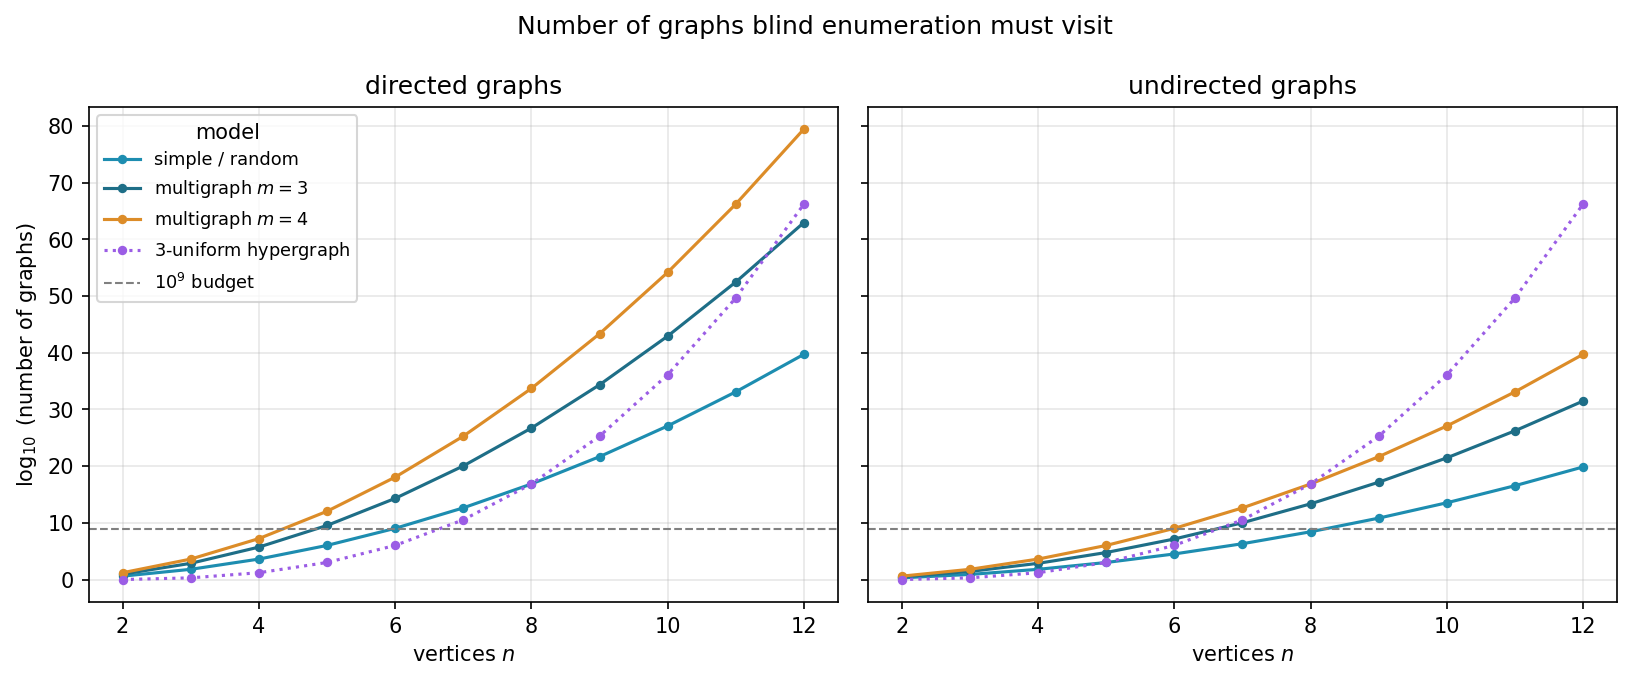
\includegraphics[width=\textwidth]{figures/complexity_growth.png}
    \caption{Candidate counts for blind enumeration on a logarithmic scale. Every model crosses the generous $10^9$ budget in single-digit order, and directed objects grow fastest because they have more independent entries to decide.}
    \label{fig:complexity}
\end{figure}

The vertex count dominates every other factor.
The candidate count has the form (values per entry)$^{\text{(number of entries)}}$.
For graphs, the number of entries grows quadratically with $n$.
For fixed-rank $r$-uniform hypergraphs, it grows as $\binom{n}{r}=\Theta(n^r)$.
The $r=3$ experiments plotted here therefore have cubic growth in the exponent.

Raising the connectivity budget enlarges the number of values available in each entry.
A simple graph has two states per entry, while a multigraph has more.
Adding direction instead increases the number of entries.
It decides both directions of a pair independently, turning two undirected states into four directed states.
Which change costs more depends on $m$ and on the model.
Directed hypergraphs are especially numerous because each hyperedge also requires a
choice of tail and heads.
These variants are particularly costly to enumerate, even where a conjecture predicts their leading term.
The separation, by contrast, does not change the enumeration: edge and vertex disjointness
start from the same candidate space, but use different feasibility tests. Their pruning and running times can therefore differ.

\begin{figure}[ht]
\centering
\begin{tikzpicture}[>=Stealth]
% ---- (a) digraph -> multiplicity matrix, diagonal highlighted, asymmetric ----
\node[vertex] (A) at (0,   0)   {$1$};
\node[vertex] (B) at (2.0, 0)   {$2$};
\node[vertex] (C) at (1.0, 1.7) {$3$};
\draw[arc] (A) to[bend left=15]  (B);
\draw[arc] (A) to[bend right=15] (B);
\draw[arc] (B) to[bend left=15]  (C);
\draw[arc] (C) to[bend left=15] (B);
\draw[arc] (A) -- (C);
\node[font=\small] at (1.0, -0.8) {directed multigraph $G$};
\node at (3.3, 0.55) {$\xrightarrow{\;\mu\;}$};
\node at (5.4, 0.55) {$\begin{pmatrix} {\color{vertexred}\mathbf 0} & 2 & 1 \\ 0 & {\color{vertexred}\mathbf 0} & 1 \\ 0 & 1 & {\color{vertexred}\mathbf 0} \end{pmatrix}$};
\node[font=\small] at (5.4, -0.8) {multiplicity matrix $\mu$};
\node[font=\scriptsize, vertexred] at (5.4, -1.3) {Diag($\mu$)$=0$ (no loops)};
% ---- (b) directed hypergraph -> list of hyperedges, tail 3 shared by both ----
\begin{scope}[yshift=-3.5cm]
  \coordinate (p1) at (0.0, 0.6);
  \coordinate (p2) at (0.0,-0.6);
  \coordinate (p3) at (1.1, 0.0);
  \coordinate (p4) at (2.2, 0.6);
  \coordinate (p5) at (2.2,-0.6);
  \begin{scope}[on background layer]
    \draw[metro, metroA, -{Stealth[length=2.6mm]}, shorten >=2mm, shorten <=1.4mm] (p3) -- (p1);
    \draw[metro, metroA, -{Stealth[length=2.6mm]}, shorten >=2mm, shorten <=1.4mm] (p3) -- (p2);
    \draw[metro, metroB, -{Stealth[length=2.6mm]}, shorten >=2mm, shorten <=1.4mm] (p3) -- (p4);
    \draw[metro, metroB, -{Stealth[length=2.6mm]}, shorten >=2mm, shorten <=1.4mm] (p3) -- (p5);
  \end{scope}
  \foreach \p/\lbl in {p1/1,p2/2,p3/3,p4/4,p5/5} {\node[smallvertex] at (\p) {$\lbl$};}
  \node[font=\small] at (1.1,-1.25) {directed hypergraph $H$};
  \node at (3.3, 0.0) {$\longrightarrow$};
  \node[font=\small, align=left] at (5.9, 0.0)
    {list of hyperedges:\\[3pt] $e_1: \{3\ |\ 1,2\}$\\[1pt] $e_2:\{3\ |\ 4,5\}$};
\end{scope}
\end{tikzpicture}
\caption{The two encodings for directed variants. The multiplicity matrix $\mu$ represents a digraph, with $\mu_{ij}$ arcs from $i$ to $j$. A list of hyperedges represents a directed hypergraph and records each tail separately. A multihypergraph repeats entries in that list. A tensor representation would require $n^r$ entries, almost all zero, and is therefore avoided.}
\label{fig:matrix-rep}
\end{figure}

The number of graphs the checker must visit grows as $2^{\binom{n}{2}}$ for simple undirected graphs and $2^{n(n-1)}$ for digraphs,
and capping multiplicities at $m-1$, so that each run ranges over the $m$ values $\{0,\dots,m-1\}$, raises the base from two to $m$,
giving $m^{\binom{n}{2}}$ undirected multigraphs and $m^{n(n-1)}$ directed ones.
The enumeration is exact wherever it finishes and it does so only for the smallest sizes.
\Cref{fig:complexity} measures exactly how fast the search space grows.

\subsection{Pruned search}
The enumeration step will skip whole families of hopeless graphs, via a pruned search.
The directed $m=2$ values are checked independently at every order through $n=7$, under both separations (\Cref{tab:basecase-search}).
\Cref{thm:dir-vertex-m2-exact,thm:dir-arc-m2-exact} propose all-order formulas whose upper-bound proofs depend on the unchecked reachability-skeleton argument. The sweep establishes only the listed finite cases.
Those orders lie just beyond the range where blind digraph enumeration is practical.
They can be reached by enumerating more cleverly.
Every variant offers a fixed list of edges its graphs are allowed to use,
whether those are pairs, ordered pairs, or oriented sets of $r$ vertices,
and a graph is a choice of how many copies each of them gets.
Rather than writing out whole choices one after another,
fix an order on that list and decide the edges one at a time,
leaving the undecided ones absent.
Each partly built graph then stands for the whole family of graphs agreeing with it so far,
and a pruning rule discards that entire family if it is deemed to bear no fruit.

Adding an edge never lowers connectivity because every existing family of disjoint routes survives (\Cref{prop:monotone}).
Every completion of a partly built graph only adds edges.
The partial graph is therefore a lower bound on the connectivity of every completion.
If it already breaks the cap, every completion does too.
The entire branch can then be abandoned.

A second pruning method starts with the edges already placed.
It then adds the largest possible contribution from the undecided edges: their number times the largest allowed multiplicity.
The resulting sum is an upper bound on every completion.
If this upper bound cannot beat the best feasible graph found so far, the branch is discarded without further exploration (\Cref{fig:prune}).
Only infeasible graphs and graphs that cannot beat the incumbent are ever discarded, so a run that finishes returns exactly the maximum the basic walk would have returned.

\begin{figure}[ht]
\centering
\begin{tikzpicture}[scale=1.0, >=Stealth,
   live/.style={gvertex, minimum size=5.5mm},
   dead/.style={gvsink, minimum size=5.5mm},
   bnd/.style={gvhub, minimum size=5.5mm},
   best/.style={gvertex, draw=vertexgreen!70!black, fill=vertexgreen!18, minimum size=5.5mm},
   br/.style={gline}]
  \node[live] (r) at (0,0) {};
  \node[live] (l) at (-2.2,-1.3) {};
  \node[live] (rr) at (2.2,-1.3) {};
  \draw[br] (r) -- node[above left, font=\scriptsize, pos=0.55]{add arc} (l);
  \draw[br] (r) -- node[above right, font=\scriptsize, pos=0.55]{skip arc} (rr);
  \node[best] (l1) at (-3.1,-2.7) {};
  \node[dead] (l2) at (-1.4,-2.7) {};
  \draw[br] (l)--(l1);
  \draw[line width=1pt, vertexred!60] (l)--(l2);
  \node[dead] (r1) at (1.3,-2.7) {};
  \node[bnd]  (r2) at (3.1,-2.7) {};
  \draw[line width=1pt, vertexred!60] (rr)--(r1);
  \draw[line width=1pt, vertexorange!70] (rr)--(r2);
  \node[font=\scriptsize, vertexgreen!50!black, align=center] at (-3.1,-3.5) {best\\feasible};
  \node[font=\scriptsize, vertexred, align=center] at (-1.4,-3.5) {infeasible\\(prune)};
  \node[font=\scriptsize, vertexred, align=center] at (1.3,-3.5) {infeasible\\(prune)};
  \node[font=\scriptsize, vertexorange!80!black, align=center] at (3.1,-3.5) {cannot beat\\best (prune)};
\end{tikzpicture}
\caption{Each level of the partially built graph fixes one adjacency. Infeasible partial graphs (red) and branches unable to beat the incumbent (orange) are discarded.}
\label{fig:prune}
\end{figure}

\subsection{Generating search}
Iterating over all possible graphs and measuring each one's connectivity repeats many isomorphic cases.
Another method, suggested by Prof.\ Jan Goedgebeur, instead generates all non-isomorphic graphs.
It uses the \texttt{geng} program from the \texttt{nauty} toolkit of McKay and Piperno \cite{McKayPiperno14}
to perform the difficult task of generating one representative of each isomorphism class.
The program is called as a subprocess, and its \texttt{graph6} output is decoded.
For a given $n$, \texttt{geng} produces all non-isomorphic \emph{undirected} graphs.
The program then treats each such graph as a support graph and assigns directed arc multiplicities to its edges.
Consequently, the search automatically inherits the support graph's isomorphism reduction.
For each support edge $\{u,v\}$, considered in a fixed order, it assigns the ordered pair
of multiplicities $\mu(u,v)$ and $\mu(v,u)$. Each lies between $0$ and $m-1$, and the two cannot both be zero because every support edge must represent at least one arc.
After each assignment, the checker evaluates the partially decorated multigraph.
If any pair already exceeds the allowed connectivity, that branch is stopped immediately:
adding more arcs cannot decrease connectivity. This is the same monotonicity-based pruning used in \Cref{fig:prune}.
Decorations that reach the target arc count are retained and converted to canonical form,
which ensures that each isomorphism class is reported only once.
Because different support graphs produce disjoint search spaces, they can be processed independently on separate processor cores.
The related orientation tools \texttt{directg} and \texttt{watercluster2} are not used.
Both allow edges in both directions, but they do not assign the repeated arc multiplicities used here \cite{NautyGuide29}. The custom decoration step also applies the connectivity pruning after each assignment.

\Cref{tab:generating-benchmark} records historical timings for three different single-core tasks. The distinction matters: they are not three equivalent ways of discovering an unknown optimum.
The blind sweep maximises the arc count over all matrix assignments.
The pruned depth-first search also maximises it, but starts with a supplied feasible construction as an incumbent.
The \texttt{geng} pipeline is given the already known extremal arc count and lists the feasible isomorphism classes at that target. Finding representatives there does not rule out a larger feasible count, so this last run does not prove the optimum independently.

The blind sweep is omitted after $n=4$, where $2^{n(n-1)}$ assignments already take $6.3$\,s.
Each additional vertex multiplies the assignment count by $2^{2n}$.
The estimated runtime is about an hour at $n=5$ and several weeks at $n=6$.
This is the growth shown in \Cref{fig:complexity}.

Below $n=5$, fixed overhead dominates the two remaining methods.
The main costs there are Python function calls and subprocess start-up.
Those timings do not give a meaningful comparison of search performance.
At $n=7$, the recorded pruned maximisation takes $1156.6$\,s and the supplied-target classification takes $17.0$\,s. Their different outputs and prior information prevent interpreting this ratio as a speed-up for proving an unknown optimum. The script gives the pruned search a $1800$-second stopping target. The blind and generated routines have no common time limit. These observations illustrate the cost of the respective tasks, not an equal-budget performance comparison.

\begin{table}[ht]
    \centering
    \small
    % Times measured on the author's machine, single core (geng parallel=False),
% directed simple digraphs, m=2. Generated classification is GIVEN the optimal
% target count and does not independently prove optimality. Blind sweep
% omitted past n=4, where 2^(n(n-1)) assignments already cost 6.3s. Each
% further vertex multiplies the assignment count by 2^(2n), and the per-
% assignment check grows too: the recorded n=3 to n=4 step cost about twice
% its count ratio. Both factors together put n=5 near an hour and n=6 at
% weeks. Reproduced by
% program/scripts/generating_search_benchmark.py against erdos915_unified.py.
\begin{tabular}{rrrrr}
\toprule
$n$ & supplied target & blind (s) & pruned (s) & classification (s) \\
\midrule
3 & 4  & 0.05 & 0.003 & 0.009 \\
4 & 6  & 6.3  & 0.008 & 0.008 \\
5 & 8  & --   & 0.22  & 0.039 \\
6 & 10 & --   & 14.5  & 0.73  \\
7 & 12 & --   & 1156.6 & 17.0 \\
\bottomrule
\end{tabular}

    \caption{Historical timings for different tasks: blind maximisation, construction-seeded pruned maximisation and \texttt{geng}-based classification at a supplied target. Only the first two independently bound the optimum from above. A dash means not attempted. These are separate runs from \Cref{tab:basecase-search}, whose recorded times differ. The table is not evidence of a like-for-like speed-up.}
    \label{tab:generating-benchmark}
\end{table}
\section{Proving every \texorpdfstring{$m$}{m} at once}

The search so far treats one pair $(n,m)$ at a time.
For a directed multigraph, scaling can instead check every threshold at a fixed $n$ in one pass.
It divides all multiplicities by $m-1$.
The formula in \Cref{thm:dir-multi-full} now supplies a lower-bound witness in \code{solve}. The cut formulation can provide a separate finite check, provided its optional cuts are valid independently of that conjecture.

Divide each multiplicity of a feasible directed multigraph $D$ by $m-1$.
The resulting weights satisfy $w(u,v)\in[0,1]$.
Every pairwise maximum flow is at most one.
Their total weight is the arc count of $D$ divided by $m-1$ (\Cref{fig:scaling-reduction}).
Let
\[
    M^{*}(n) = \max\Bigl\{\textstyle\sum_{u \ne v} w(u, v) : w(u,v) \in [0,1], \ \mathrm{maxflow}(s, t; w) \le 1 \ \text{for all } s \ne t\Bigr\}
\]
denote the largest total weight of such a matrix.
Scaling then gives
\[
    L_m^{\mathrm{dir}}(n) \;\le\; (m - 1)\, M^{*}(n)
    \qquad \text{for every } m \ge 2 .
\]

The reverse inequality needs a $\{0,1\}$ matrix of weight $M^{*}(n)$.
Multiplying such a matrix by $m-1$ preserves integer arc multiplicities.

On the linear branch, \Cref{const:dir-multi-lower} supplies the double star.
It has one hub joined bidirectionally to every other vertex and has $2(n-1)$ arcs.
For $n\le6$, this is the larger term of $M(n)$ and realises $M^{*}(n)$.
At the crossover $n=7$, the quadratic branch catches the linear one (\Cref{thm:dir-arc-m2-exact}).
It then overtakes it.
The relevant construction becomes the one-directional bipartite digraph from \Cref{const:dir-multi-lower}.
Thus no single shape witnesses $M^{*}(n)$ at every order.

What would generalise is integrality.
\Cref{cor:mstar-integral} proposes that some $\{0,1\}$ matrix always attains $M^{*}(n)$, and that this optimum equals $M(n)$.
An explicit construction gives attainment from below.
Clearing denominators from a rational optimum reduces the reverse inequality to \Cref{thm:dir-multi-full}, whose proposed proof is unchecked, so the identity below inherits that dependency.
Scaling the integral maximiser by $m-1$ gives the lower bound $(m-1)M^{*}(n)$.
The preceding scaling argument gives the matching upper bound unconditionally.
The finite optimisation is retained only as an independent check of the cases $n\le6$, and \Cref{sec:transcripts} records what it ran.
\[
    L_m^{\mathrm{dir}}(n) = (m - 1)\, M^{*}(n)
    \qquad \text{for every } m \ge 2 .
\]
\begin{figure}[ht]
\centering
\begin{tikzpicture}[>=Stealth, font=\small]
    % Left: integer multigraph (m=3), multiplicities in {0,1,2}
    \node[vertex] (A1) at (-4.2, 0)   {$A$};
    \node[vertex] (B1) at (-2.4, 1.1) {$B$};
    \node[vertex] (C1) at (-2.4,-1.1) {$C$};
    % A->B multiplicity 2: two parallel arcs
    \draw[->, arc] (A1) to[bend left=22]  node[above, font=\scriptsize]{$2$} (B1);
    \draw[->, arc] (A1) to[bend right=5]  (B1);
    % A->C multiplicity 1
    \draw[->, arc] (A1) -- node[below, font=\scriptsize]{$1$} (C1);
    % B->C multiplicity 0: absent (dotted, grayed out)
    \draw[->, arc, color=gray!50, dashed] (B1) -- node[right, font=\scriptsize, color=gray!60]{$0$} (C1);
    \node[above, font=\footnotesize\itshape] at (-3.3, 1.8) {multigraph ($m=3$)};

    % Scaling arrow
    \draw[->, very thick] (-1.2, 0) -- (1.2, 0);
    \node[above, font=\small] at (0, 0.1) {$\div\,(m-1)\;=\;\div\,2$};

    % Right: weight matrix, weights in [0,1]
    \node[vertex] (A2) at (2.4, 0)   {$A$};
    \node[vertex] (B2) at (4.2, 1.1) {$B$};
    \node[vertex] (C2) at (4.2,-1.1) {$C$};
    % A->B weight 1
    \draw[->, arc] (A2) -- node[above, font=\scriptsize]{$1$} (B2);
    % A->C weight 1/2
    \draw[->, arc] (A2) -- node[below, font=\scriptsize]{$\tfrac{1}{2}$} (C2);
    % B->C weight 0: absent
    \draw[->, arc, color=gray!50, dashed] (B2) -- node[right, font=\scriptsize, color=gray!60]{$0$} (C2);
    \node[above, font=\footnotesize\itshape] at (3.3, 1.8) {weight matrix ($M^*$)};
\end{tikzpicture}
\caption{Scaling at $m=3$: dividing multiplicities by $m-1=2$ turns the integer multigraph into a weight matrix with entries in $[0,1]$ and pairwise maximum flow at most one. Hence one $m$-free optimisation bounds every threshold.}
\label{fig:scaling-reduction}
\end{figure}

\section{The heuristic search}
So far, iterating all graphs of a fixed size that meet the connectivity constraint and counting their edges was a blind walk.
Apart from pruning, there is nothing that steers the walk towards better candidates because they all need to be checked anyway.
From a certain point onwards, that will become impossible due to the massive number of possible graphs.
The goal then becomes finding the densest possible graphs in such an efficient and guided way that they are
likely to be (almost) extremal.
The guide that pulls the walk towards a (local) maximum is called a heuristic.
To avoid getting stuck in a local maximum, a metaheuristic allows worsening moves to discover new optima.

For graph and digraph models represented by a multiplicity matrix, give each candidate one number: its energy
\[
    \Phi(G) = -|E(G)| + \Lambda \cdot \max\bigl(0,\ c^{\max}(G) - (m - 1)\bigr),
\]
which rewards edges or arcs and penalises any excess connectivity, where $c^{\max}(G)$ denotes $\lambda^{\max}(G)$ or $\kappa^{\max}(G)$, matching whichever separation the run measures.
The matrix search starts from the empty graph and changes one edge or arc multiplicity by one at each move.
The method used is \emph{tabu search} \cite{Glover89},
which escapes a local optimum by forbidding the pairs it has just touched.
Among the moves not forbidden, the walk always takes the one that lowers $\Phi$ most, even when every candidate raises it.
This is unlike a greedy walk that only ever accepts an improving move.
After each move the pair it changed is put on a tabu list for a fixed number of steps,
so the walk cannot immediately undo what it just did and cycle back into the optimum it came from.
A move that would beat the best graph seen so far overrides the tabu flag regardless of its status,
an \emph{aspiration criterion} that keeps the tabu list from ever blocking genuine progress,
and the walk perturbs itself when it stalls.

Simulated annealing is an alternative on the same energy and neighbourhood \cite{KirkpatrickGelattVecchi83}.
It accepts worsening moves with the probability given by the Metropolis rule \cite{Metropolis53}.
That probability decreases as the run cools.
At an equal wall-clock budget, annealing is the weaker engine here.
For $n=7$ and $m=3$, tabu reaches the $24$-arc directed multigraph construction, while annealing reaches $20$ arcs.
For the simple digraph, tabu reaches $18$ arcs and annealing reaches $16$.
Matrix-model discovery uses tabu search. Supplied constructions are reported separately from the search outcomes.
Annealing is retained for the comparison above and as an independent cross-check in the program's self-test,
where agreement between two unrelated walks is worth more than the speed of either.

Allowing the walk above the cap is a search strategy, not a requirement for reaching every feasible graph.
Removing an edge can only lower $\lambda^{\max}$ and $\kappa^{\max}$, never raise them,
so every subgraph of a feasible graph is again feasible, and the empty graph is feasible trivially.
From any feasible target we can therefore delete edges one at a time down to the empty graph
without ever crossing the cap, and reading that path backward builds the target up the same way.
The feasible region is connected through the empty graph by single-edge moves that stay inside it,
so a walk that never went infeasible could in principle visit every feasible graph there is.
We let the walk become infeasible because reachability and efficiency are different questions.
A feasible graph can be locally maximal even when it is far from globally optimal.
Escaping it may require exchanging one edge for another.
Removing first and then adding stays feasible, but the removal temporarily worsens the objective.
Reversing the order keeps the edge count high, but the addition may temporarily violate the connectivity cap.
Allowing both orders gives the walk another short route across a local barrier.
Infeasibility is a search device, not a target.
A single walk depends on its starting point and random seed.
The program therefore runs several independent restarts until the wall-clock budget expires.
It keeps the densest witness found by any restart.
The restarts share no state and can run on separate processor cores.

\subsection{Random greedy growth for hypergraphs}

Hypergraph discovery uses a separate random greedy procedure. Each restart
begins with the empty hypergraph and a shuffled list of all permitted hyperedge
types. The list contains one occurrence of each type in the simple model and
$m-1$ occurrences in the multihypergraph model. Directed candidates retain
their tail and head sets. The procedure tries each occurrence in turn, keeps
the added copy if the exact Berge-connectivity checker returns at most $m-1$,
and otherwise removes that copy. It repeats with a new shuffled order until
the time budget expires, retaining the densest feasible result.

A completed pass is maximal under adding one copy: every rejected copy was
already infeasible when tried, and later additions cannot reduce connectivity
(\Cref{prop:monotone}). Maximality does not imply maximum size. An early choice
can prevent several later choices, and this procedure makes no exchanges or
temporarily infeasible moves within a pass. The shuffled restarts explore
different choices. An interrupted pass still supplies a feasible lower bound.

The current tabu engine changes entries of a multiplicity matrix and is not
implemented for the hyperedge-list representation. Extending it would require
hyperedge moves and corresponding tabu bookkeeping. A full neighbourhood scan
would consider $\binom{n}{r}$ types in an undirected simple hypergraph and
$r\binom{n}{r}$ in the forward directed model, with feasibility measured in
the expanded gate network. This motivates the simpler implementation, but
does not establish a performance advantage: no hypergraph tabu comparison was
run. The equal-allocation experiment below compares the implemented searches,
including their different methods.

\subsection{Measuring only near the connectivity cap}
Removing an edge, arc, or hyperedge can never raise $\lambda^{\max}$, while adding one raises it by at most one.
The same holds for $\kappa^{\max}$.
This relies on the monotonicity and unit-step bounds of \Cref{prop:monotone}.
Therefore the max-flow algorithm only needs to be run every once in a while,
depending on how close to the constraint the graph sits.
Most steps need no measurement at all.
A removal from a feasible graph leaves it feasible.
An addition made while the graph sits strictly below the cap lifts
$\lambda^{\max}$ by at most one, so it lands at worst on the cap.
Every other step calls the checker.
There are two of those: an addition whose running bound sits at or above
the cap, and a removal from a graph already above it.
The search keeps that running bound and raises it by one for each addition
it accepts.
At a fixed step interval it measures the exact value again.
\Cref{sec:cheap-checker} gives the bookkeeping,
and the regression test that holds the fast walk to the naive one step for step.

\section{An equal search allocation across all variants}\label{sec:equal-budget}

A separate experiment gives each of the sixteen variants one hour of search
in total. This is one hour per variant, not per parameter case. Each variant
is tested at $n=6,8,10,12$ and $m=3,6$. Each of these eight cases receives
three runs with initial seeds $0$, $1000000$ and $2000000$, each with a
$150$-second stopping target. Thus every variant receives
$8\cdot3\cdot150=3600$ seconds of allocated search.

All runs start empty. No construction, known optimum or earlier incumbent is
supplied to the search. Graph variants use tabu search and hypergraph variants
use random greedy growth. Hypergraphs have rank $3$ and directed hypergraphs
use the forward convention. Runs are serial, with the variant order rotated
between cases. Validation and reporting take place outside the search budget.

The original solver used a calendar clock for its stopping rule. Nineteen runs
had a discrepancy between that clock and the independently measured monotonic
duration. They are retained in the data but excluded from equal-budget
statistics. Each flagged trial was repeated with the same frozen search code
and seed, changing only its deadline clock to a monotonic one. The replacement
takes its original slot regardless of which run found more edges. Selecting
the better of the two would give those slots an unfair additional chance.
The discarded attempts are counted separately as extra computation.

The timing rule is cooperative, so a connectivity calculation already in
progress can overrun its target. Monotonic time also has platform-specific
behaviour during system suspension. The records therefore include calendar
duration, monotonic duration and CPU time. The computer was not isolated from
other work, so this is a comparison under equal allocated search durations,
not a controlled comparison of processor efficiency.

\Cref{tab:equal-budget-summary} compares the unaided outcomes with a separately
supplied construction count $C$. Reaching $C$ need not mean reaching the
optimum. Failing to reach it measures a limitation of these particular runs,
not a failure of the construction. The detailed tables in
\Cref{sec:equal-budget-details} retain the minimum, median and maximum across
the three seeds instead of replacing a search value by $C$.

\begin{table}[htbp]
\centering
\scriptsize
\begin{tabular}{lrr}
\toprule
Variant & Best reaches $C$ & All seeds reach $C$ \\
\midrule
simple graph, undirected, edge & 8/8 & 7/8 \\
simple graph, undirected, vertex & 8/8 & 8/8 \\
simple graph, directed, arc & 3/8 & 3/8 \\
simple graph, directed, vertex & 3/8 & 3/8 \\
multigraph, undirected, edge & 8/8 & 8/8 \\
multigraph, undirected, vertex & 4/8 & 4/8 \\
multigraph, directed, arc & 2/8 & 2/8 \\
multigraph, directed, vertex & 2/8 & 1/8 \\
simple hypergraph, undirected, edge & 5/8 & 4/8 \\
simple hypergraph, undirected, vertex & 5/8 & 4/8 \\
simple hypergraph, directed, arc & 4/8 & 4/8 \\
simple hypergraph, directed, vertex & 4/8 & 4/8 \\
multihypergraph, undirected, edge & 5/8 & 4/8 \\
multihypergraph, undirected, vertex & 5/8 & 4/8 \\
multihypergraph, directed, arc & 4/8 & 4/8 \\
multihypergraph, directed, vertex & 4/8 & 4/8 \\
\bottomrule
\end{tabular}

\caption{Eight parameter cases per variant under a one-hour total search
allocation. The first count records cases where the best of three seeds
reaches or exceeds the supplied construction count $C$. The second requires
all three seeds to do so. Neither column counts proved optima.}
\label{tab:equal-budget-summary}
\end{table}

\begin{samepage}
Across the $128$ parameter cases, the best run reaches or exceeds $C$ in $74$
cases and falls short in $54$. All three seeds reach $C$ in $68$ cases. In
$8$ cases the search improves on the supplied construction, which confirms
why $C$ is a comparison value rather than an asserted optimum.
The limitations are substantial in some directed models. For example, at
$n=12$ and $m=6$ the directed multigraph arc search returns $110$ in every
run, while the supplied construction has $180$ arcs. Thus the successful
small validation cases below do not imply reliable recovery of the dense
families at larger orders.\par
\end{samepage}

The selected runs used $57657.7$ seconds of measured monotonic search time
against the $57600$-second total allocation. Including the discarded originals
raises the saved search time to $58690.8$ seconds. These totals exclude
validation and reporting and are not calendar durations of the experiment.

\section{Rediscovering the known extremisers}\label{sec:rediscovery}

Before addressing open cases, the search is tested on settled ones.
Each run starts from the empty graph.
The search is given the edge-count objective and the connectivity cap, and retains only feasible witnesses. Its intermediate states may be infeasible.
It receives no description of the known extremal construction.
In all seven validation cases in \Cref{tab:rediscovery}, it reaches the established value. This is a statement about those runs, not a claim that it succeeds at every size or throughout the sixteen-variant grids.
\Cref{tab:rediscovery} compares the densest witness with the theoretical value.

\begin{table}[ht]
    \centering
    \small
    \begin{tabular}{lrrrrrr}
\toprule
Variant & $n$ & $m$ & Limit (s) & Elapsed (s) & Search & Optimum \\
\midrule
simple undirected & 6 & 2 & 2 & 2.006 & 5 & 5 \\
multi undirected & 6 & 3 & 2 & 2.004 & 10 & 10 \\
simple directed & 4 & 2 & 2 & 2.000 & 6 & 6 \\
simple directed & 6 & 2 & 2 & 2.020 & 10 & 10 \\
simple directed & 7 & 2 & 2 & 2.022 & 12 & 12 \\
multi directed & 4 & 3 & 2 & 2.000 & 12 & 12 \\
multi directed & 5 & 3 & 2 & 2.011 & 16 & 16 \\
\bottomrule
\end{tabular}

    \caption{Seven short validation runs. Each uses unaided tabu search, initial seed zero and a two-second stopping target per case. Elapsed times include the search and may slightly exceed the target because deadline checks are cooperative. The search count and known optimum are separate columns. These are not one-hour benchmarks.}
    \label{tab:rediscovery}
\end{table}

\begin{figure}[ht]
\centering
\resizebox{\textwidth}{!}{%
\begin{tikzpicture}[>=Stealth]
  % Panel 1: spanning tree, undirected simple, n=6, m=2, ell_2(6)=5
  \begin{scope}[shift={(-7.5,0)}]
    \foreach \i/\x in {1/0,2/1.0,3/2.0,4/3.0,5/4.0,6/5.0} {
      \node[gvertex, minimum size=5mm] (t\i) at (\x,0) {};
    }
    \foreach \i/\j in {1/2,2/3,3/4,4/5,5/6} {
      \draw[gline] (t\i) -- (t\j);
    }
    \node[font=\footnotesize\itshape] at (2.5,-0.9) {example tree: the path $P_6$};
    \node[font=\scriptsize] at (2.5,-1.4) {$n=6$, $\ell_2(n)=5$};
  \end{scope}
  % Panel 2: undirected multigraph star, n=6, m=3, every spoke doubled, L_3(6)=10
  \begin{scope}[shift={(0,0.3)}]
    \node[gvhub, minimum size=6mm] (h2) at (0,0) {};
    \foreach \ang in {90,162,234,306,18} {
      \node[gvertex, minimum size=5mm] (l2\ang) at (\ang:1.5) {};
      \draw[gline] (h2) to[gcurve]  (l2\ang);
      \draw[gline] (h2) to[gcurveR] (l2\ang);
    }
    \node[font=\footnotesize\itshape] at (0,-2.0) {multigraph star};
    \node[font=\scriptsize] at (0,-2.5) {$n=6$, $m=3$, $L_3(n)=10$};
  \end{scope}
  % Panel 3: directed multigraph double star, n=4, m=3, every spoke bidirected and doubled, L_3^dir(4)=12
  \begin{scope}[shift={(5.2,0.3)}]
    \node[gvhub, minimum size=6mm] (h3) at (0,0) {};
    \foreach \ang in {90,210,330} {
      \node[gvertex, minimum size=5mm] (l3\ang) at (\ang:1.9) {};
      \draw[gdir] (h3)     to[bend left=30]  (l3\ang);
      \draw[gdir] (h3)     to[bend left=11]  (l3\ang);
      \draw[gdir] (l3\ang) to[bend left=30]  (h3);
      \draw[gdir] (l3\ang) to[bend left=11]  (h3);
    }
    \node[font=\footnotesize\itshape] at (0,-2.4) {double star};
    \node[font=\scriptsize] at (0,-2.9) {$n=4$, $m=3$, $L_3^{\mathrm{dir}}(n)=12$};
  \end{scope}
\end{tikzpicture}%
}
\caption{Examples from the extremal families discussed alongside \Cref{tab:rediscovery}, drawn at the reported sizes. The path illustrates the tree family but is not the saved search witness. \Cref{fig:simple-digraph-m2} shows a bidirected star, which ties the one-directional wall at $n=7$.}
\label{fig:rediscovery-gallery}
\end{figure}

The recorded witnesses can be inspected, rather than inferring their shapes from their edge counts. They are saved with methods and elapsed times in \code{program/data/rediscovery.json}. \code{program/scripts/rediscovery.py} runs the experiment and \code{make\_figures.py} renders the table without rerunning it. Each later restart uses the next integer seed. The supplied optimum is not passed to the search. All seven saved witnesses have star-shaped support, with the direction and multiplicity specified below.
\Cref{fig:rediscovery-gallery} draws three examples.
The undirected simple run at $m = 2$ settles on a tree. The example drawn is the path $P_6$.
Every tree on $n$ vertices has $n-1$ edges and local edge-connectivity at most one.
The search therefore recovers an extremal family rather than a unique shape.

The undirected multigraph run settles on a star whose spokes have multiplicity $m-1$.
This is an instance of the multi-tree extremiser of \Cref{thm:multigraph-edge}.
The directed multigraph run finds the same star with both directions present at that multiplicity.
It is the thickened tree of \Cref{const:dir-multi-lower}.

The simple directed run finds a bidirected star at $n=4$.
At $n=7$ it finds twelve arcs, where the hub and the one-directional wall tie (\Cref{fig:simple-digraph-m2}).
This is the crossover predicted by \Cref{thm:dir-arc-m2-exact}.
The search carries none of these names.
It finds the constructions solely by optimising under the connectivity cap.

The seven successful cases do not establish reliable performance past $n=7$.
At $n=8$ and $m=2$, a bidirected star has fourteen arcs, whereas a one-directional balanced wall has sixteen.
Moving from a completed hub to the one-directional wall requires many coordinated arc changes (\Cref{fig:simple-digraph-m2}).
Single-arc moves can therefore make the star a difficult state to escape. This explains a possible search obstruction, not a proof that every run must stall there.
The explicit construction and its connectivity check supply the sixteen-arc lower bound independently of whether an unaided run finds it.

The double star of \Cref{fig:rediscovery-gallery} provides another witness beyond the search range.
At $n=7$ and $m=4$, it has $36$ arcs and $\lambda^{\max}=3$.
Its count equals $2(n-1)(m-1)$.
Neither witness alone proves optimality.
Each is an exactly measured feasible graph and therefore a lower bound.
